\documentclass[12pt,a4paper]{report}
\setlength\textwidth{145mm}
 \setlength\topmargin{0mm}
 \setlength\headsep{0mm}
 \setlength\headheight{0mm}
 
% Přepneme na českou sazbu
\usepackage[czech]{babel}
\usepackage[IL2]{fontenc}
\usepackage{graphicx} 

%% Použité kódování znaků: obvykle latin2, cp1250 nebo utf8:
\usepackage[utf8]{inputenc}
\begin{document}


\section{Rovnoměrný vs nevyvážený test}
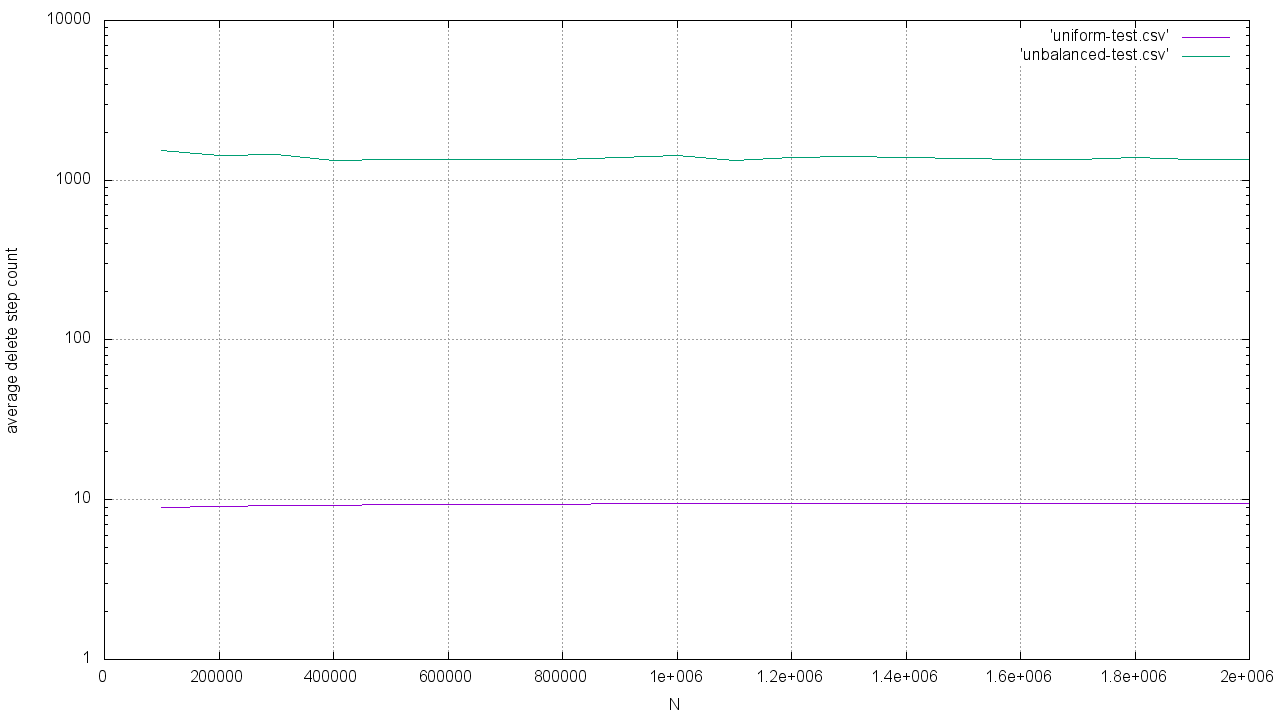
\includegraphics[width=\textwidth]{./tests/graph1.png}

Jak je vidět na předchozím grafu pro nevyvážený test se provádí mnohem 
více konsolidací. To je způsobeno tím, že se v tomto testu provádí více operací decrease-key,
které potom vytvářejí mnohem víc stromů, které musí být následně zkonsolidovány. 

\section{Standartní vs naivní implementace}
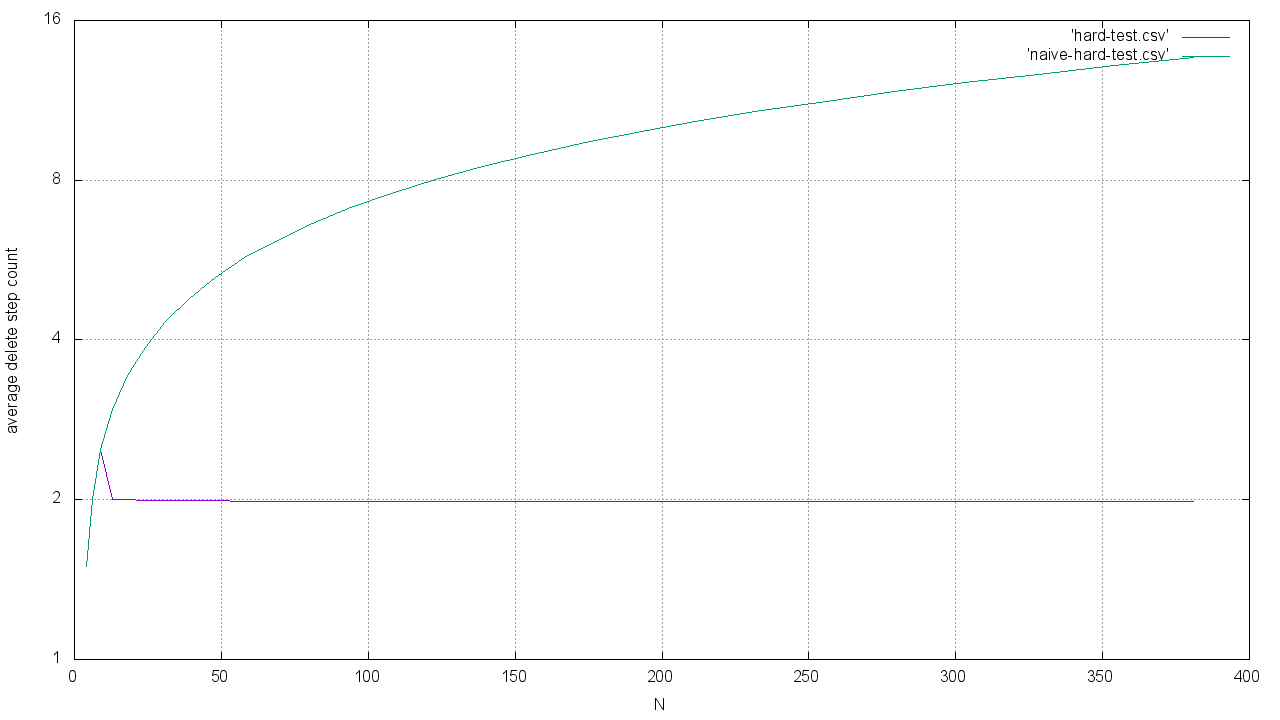
\includegraphics[width=\textwidth]{./tests/graph2.png}


  
\end{document}